
\chapter{Future Improvements - Vector Boson Fusion HH Production}

To improve this analysis, a signal model for the Vector Boson Fusion production mode has been designed and will be implemented into this analysis using the full ``Run 2'' dataset. This signal model is integrated into the analysis through a separate analysis category that is enriched in VBF events, defined via cuts on multiclass \gls{BDT} scores.

\section{Simulated Samples}

\subsection{Non-resonant VBF HH Samples}

The signal MC samples for VBF $HH$ production are generated at LO using \MGMCatNLO 2.6.0, using cards presented in \cite{vbfhh}. The process generated is $pp \rightarrow HHqq$. The dominant production in this sample is VBF $HH$ production, but contains contributions from $VHH$  hadronic and Higgsstrahlung production. The NNPDF 2.3 LO PDF set \cite{NNPDF} is used in the matrix element, interfaced to \HERWIG 7.0.4 using the H7-UE-MMHT tune for underlying events and the H7-MMHT2014LO tune for parton shower and hadronization.

Samples have been produced for the various coupling values shown in Table \ref{tab:vbf-coupling-samples}. The values of $\kappa_\lambda$,$c_{2V}$, and $c_{v}$ are all 1 in the SM. The values selected for production aim to vary each coupling value enough that interpolation may be performed, and one value was produced near where limits could be expected to be set ($\kappa_\lambda = 10$ and $c_{2V}=4$).

\begin{table}[htbp]
    \centering
    \caption{Grid of coupling values used in production of VBF $HH$ samples.}
    \begin{tabular}{c|c|c}
        $\kappa_\lambda$ & $c_{2V}$ & $c_{v}$ \\
        \hline
        1 & 0 & 0.5 \\
        1 & 1 & 0.5 \\
        0 & 0 & 1 \\
        1 & 0 & 1 \\
        1 & 0.5 & 1 \\
        1 & 0 & 0.5 \\
        1 & 1 & 1 \\
        1 & 1.5 & 1 \\
        1 & 2 & 1 \\
        1 & 4 & 1 \\
        0 & 1 & 1 \\
        2 & 1 & 1 \\
        10 & 1 & 1 \\
        1 & 1 & 1.5
    \end{tabular}
    \label{tab:vbf-coupling-samples}
\end{table}

Relevant distributions for validation of these samples can be seen in Figure \ref{fig:vbf-mc-validation}. Plots are shown at parton level, with a basic jet selection applied to isolate the VBF jets similar to that done at reconstruction level. Jets are considered if they have $\pt > 25$, then the $m_{bb}$ pair is selected as the two jets with $m_{bb}$ closest to 125 \GeV. The VBF jets are selected as the highest $m_{jj}$ pair after removing jets used in the $m_{bb}$ pairing. Additional detail on the validation for these samples is outlined in Ref. \cite{mc-validation}.

\begin{figure}[htbp]
    \centering
    \subfloat{
      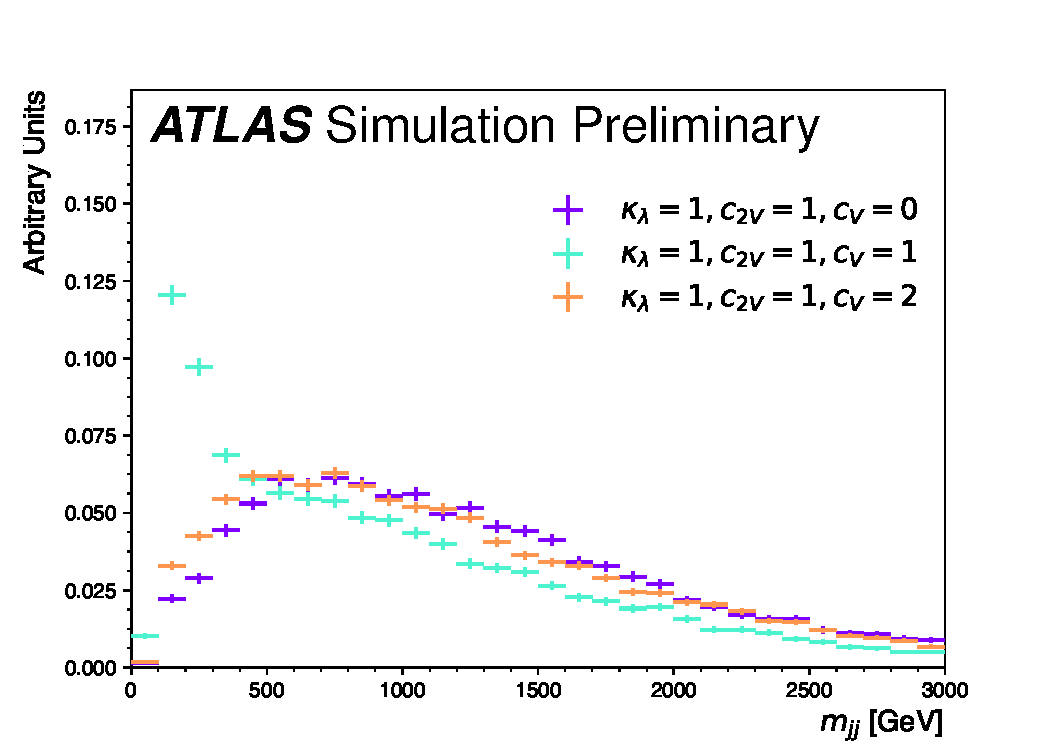
\includegraphics[width=0.33\textwidth]{chapters/chapter6_vbf/images/mc_samples/m_jj_cv.pdf}
    }
    \subfloat{
      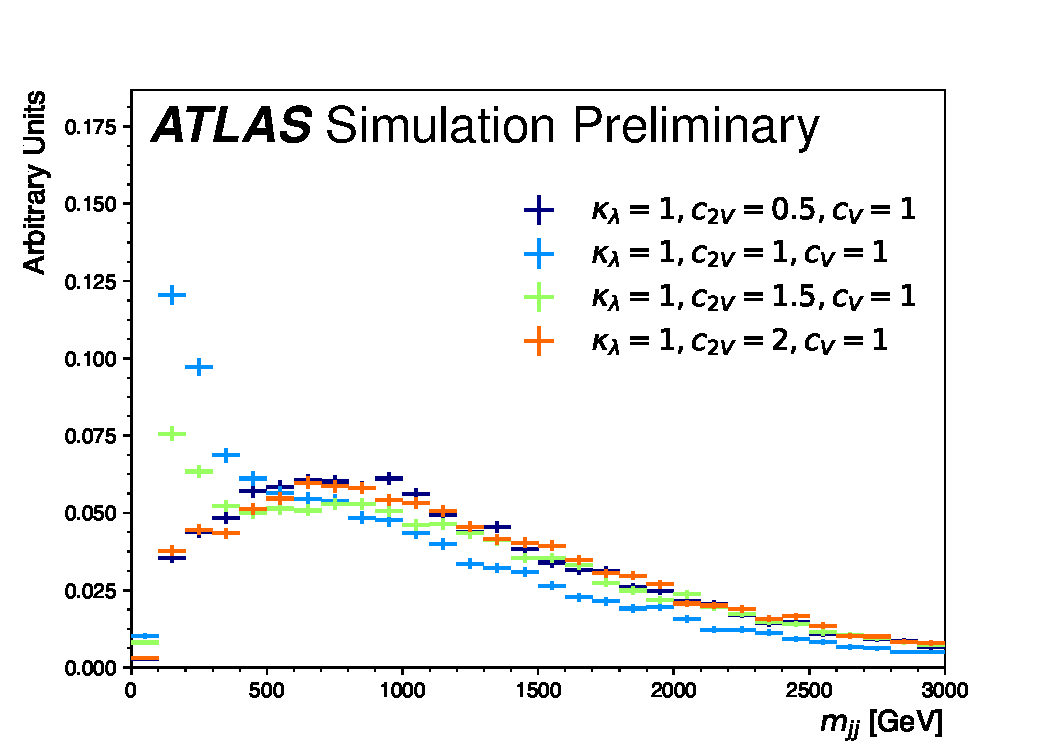
\includegraphics[width= 0.33\textwidth]{chapters/chapter6_vbf/images/mc_samples/m_jj_cvv.pdf}
    }
    \subfloat{
      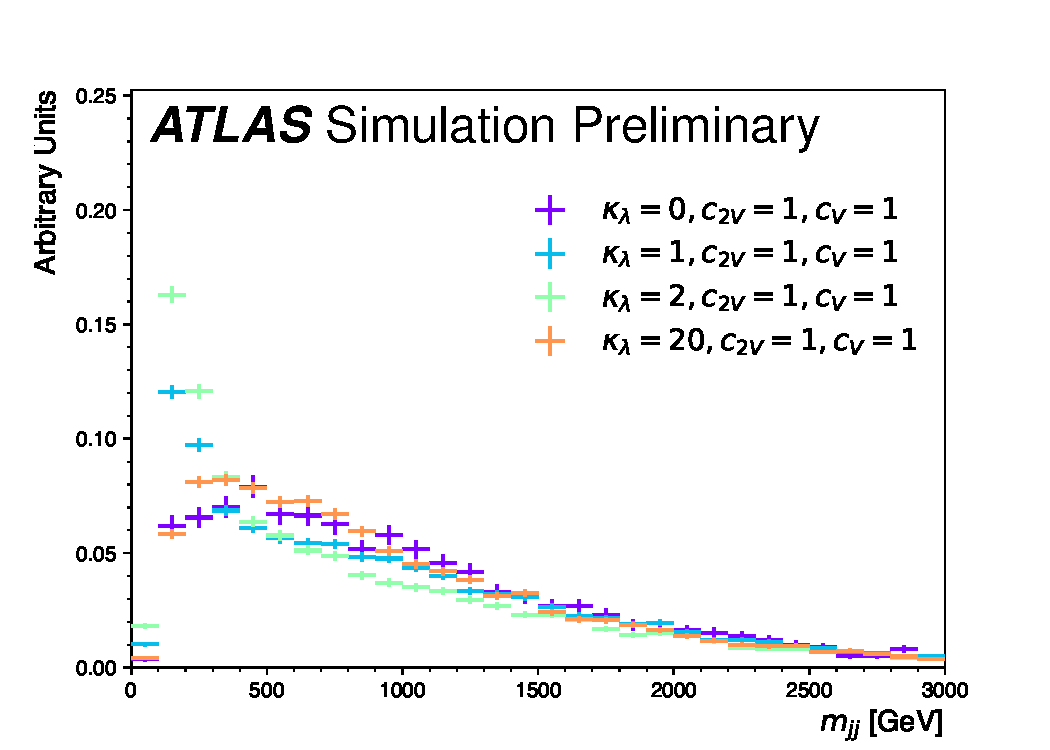
\includegraphics[width= 0.33\textwidth]{chapters/chapter6_vbf/images/mc_samples/m_jj_klambda.pdf}

    }       

    \subfloat{
        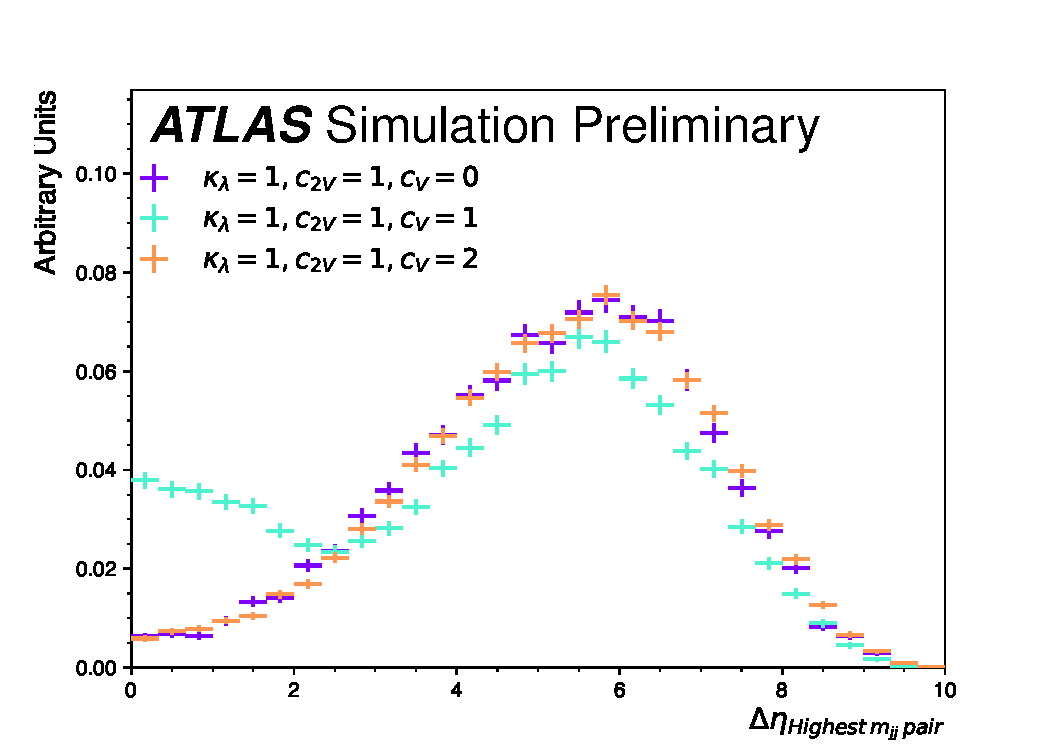
\includegraphics[width=0.33\textwidth]{chapters/chapter6_vbf/images/mc_samples/jj_deta_cv.pdf}
      }
      \subfloat{
        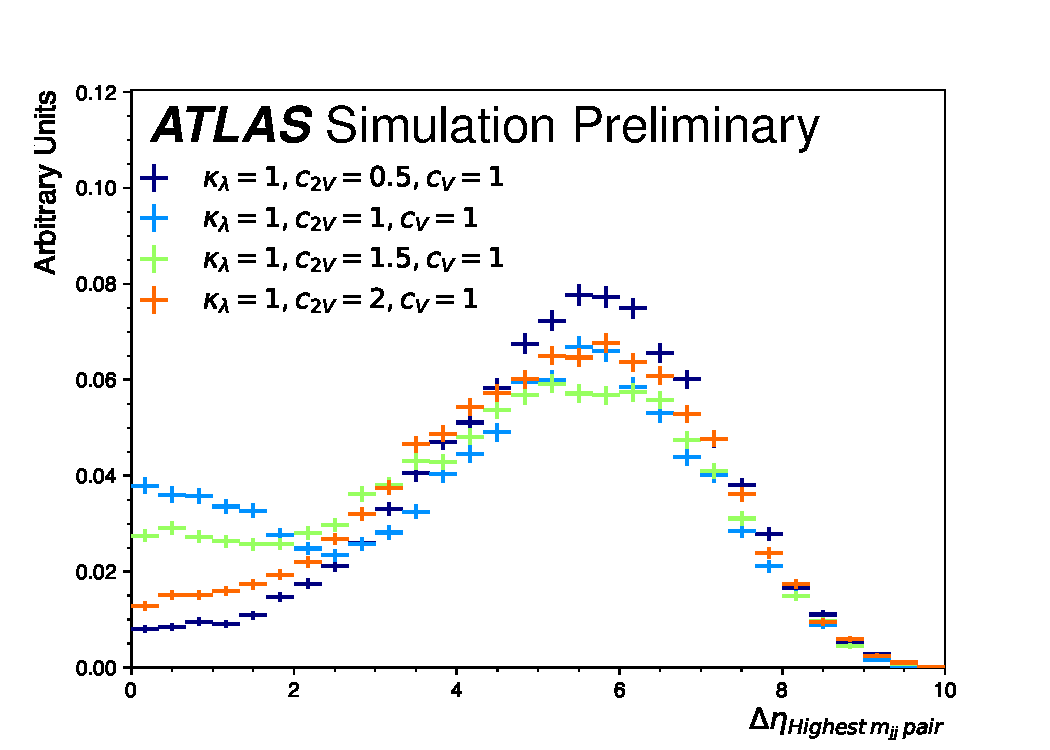
\includegraphics[width= 0.33\textwidth]{chapters/chapter6_vbf/images/mc_samples/jj_deta_cvv.pdf}
      }
      \subfloat{
        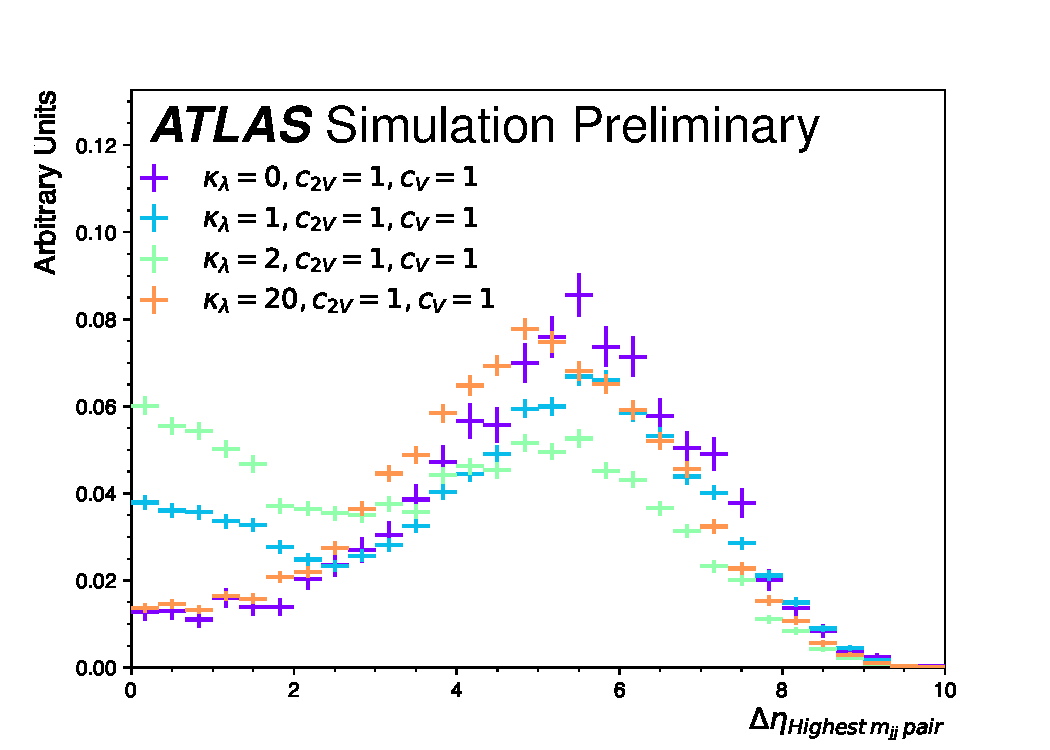
\includegraphics[width= 0.33\textwidth]{chapters/chapter6_vbf/images/mc_samples/jj_deta_klambda.pdf}
    }    

    \caption{Validation plots at parton level for the VBF $HH$ signal sample. The highest $m_{jj}$ pair is selected as a proxy for the VBF jets. The top row shows the invariant mass distribution of this system, the bottom depicts the $\Delta \eta$ between these jets. Left to right, these plots vary the $c_V$, $c_{2V}$, and $\kappa_\lambda$ strength. The peak at low $m_{jj}$ values and shoulder at low $\Delta \eta$ is a product of the $VHH$ hadronic and Higgsstrahlung contributions in the samples.}
    \label{fig:vbf-mc-validation}
\end{figure}

\section{Event Selection} \label{ssec:vbf-event-selection}

To improve the event selection presented in Section \ref{sec:yybb-event-selection} the following method is applied:

First, the following preselection cuts are applied:

\begin{itemize}
	\item $N_{\text{cen jets}}$ < 6, to help reject ttH production (hadronic top decays)
	\item $N_{\text{lep}}$ = 0, to help reject ttH production (leptonic top decays)
	\item $N_{\text{85 \% b-tags}}$ >= 2 
	\item $N_{\text{70 \% b-tags}}$ < 3, to maintain orthogonality with the HH -> bbbb analysis
\end{itemize}

\noindent\textbf{BDT for ggF Production}\\
\indent A \gls{BDT} has been trained in order to maximize signal efficiency for ggF HH production. Following preselection, events are segmented into two regions, a high mass region with $M_X^{*} > 350 \text{GeV}$ targeting the standard model signal, and a low mass region with $M_X^{*} < 350 \text{GeV}$ targeting BSM signals. 

In each region, a separate BDT is trained using a benchmark HH signal against a combination of \yy, $ttH$, $ggH$, and $ZH$ backgrounds. In the high mass region, the standard model HH sample is used as signal, while in the low mass region, the $\klambda = 6$ sample is used as signal.

The following inputs are used:

\begin{itemize}
	\item{The $p_{T}/m_{\yy}$, $\eta$, $\phi$ of the two photons} 
	\item{The $p_{T}$, $\eta$, $\phi$, and pseudo-continuous b-tagging score of the first two jets}
	\item{The MET and the $\phi$ angle of the MET}
	\item{The $p_{T}$, $\eta$, $\phi$, and mass of the $H\rightarrow \bb$ candidate}
	\item{The $H_{T}$ (scalar $p_{T}$ sum of all jets)}
\end{itemize}

Where,

\begin{itemize}
	\item{The $p_{T}$ of the two photons are scaled by $m_{\yy}$ to prevent the BDT from learning the $m_{\yy}$ variable. There is no equivalent scaling done for the two jets, since nominally we only fit to $m_{\yy}$, not $m_{\bb}$.}
	\item{Jets are ordered by pseudo-continuous b-tagging score, and then by $p_{T}$ in case of a tie. The $H \rightarrow \bb$ candidate is then formed by the two highest ranked jets by simply summing their four-vectors.}
	\item{All vectors are rotated by the same $\phi$ angle so that the $\phi$ of the leading photon is equal to zero. This effectively removes one degree of freedom for the BDT to learn.}
\end{itemize}

After training, two categories are created in each mass region by creating cuts on the BDT output. The category boundaries are optimized to give the best Asimov number counting significance \cite{asimov}, given by

\begin{equation}\label{eqn:asimov-significance}
    Z = \sqrt{2[(s+b)\log{(1 + s/b)} -s]}.
\end{equation}


\noindent\textbf{BDT for VBF Production}\\
\indent Atop this selection, a dedicated VBF-enriched analysis category is built. Events which have already passed the ggF BDT based selection and have at least 4 jets are considered the VBF category. The 4 jet requirement is imposed in order to reconstruct VBF-based variables, since 2 jets are needed for the \Hbb decay, and another 2 are needed for the VBF jets. The VBF jets are then selected as the highest $m_{jj}$ pairing, excluding $H\rightarrow b\bar{b}$ candidate jets.

These events are then evaluated by a multiclass BDT, which has independent classes for VBF HH, ggF HH, $\gamma \gamma$-continuum, and $ttH$. Ultimately, an event selected for the VBF category if it passes the BDT score threshold for VBF HH, and fails the score threshold for the other three classes. The thresholds are determined by a 4-dimensional scan over cuts on the BDT score, with the Asimov significance as the figure of merit.

A flowchart of this logic is shown in Figure \ref{fig:vbf-logic}.

\begin{figure}[htbp]
    \centering
	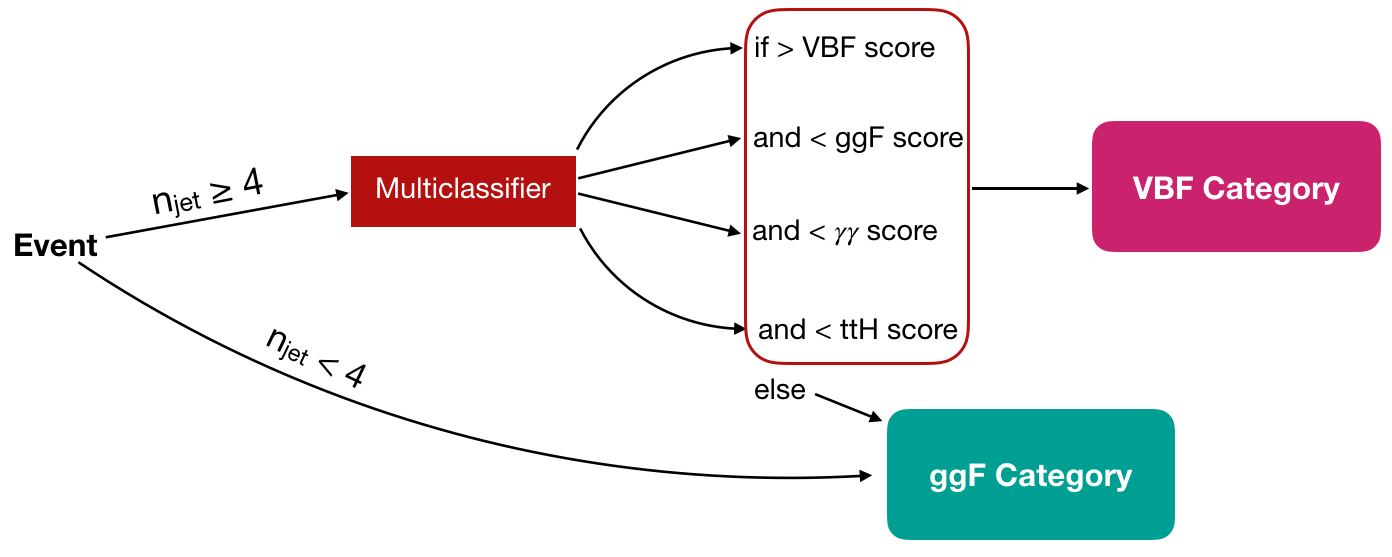
\includegraphics[width=0.9\textwidth]{chapters/chapter6_vbf/images/vbf_logic.png}
    \caption{Logic flow for an event to be selected into the VBF-enriched signal region. The starting set of candidates (denoted ``event'') requires passing preselection and at least one of the ggF-based signal categories. If an event is assigned to the ggF categories, it is separated into 4 categories.}
    \label{fig:vbf-logic}
\end{figure}


\begin{center}
	\begin{tabular}{c|c|c}
	\hline
	Class & Target & Selection Logic  \\
	\hline
	0 & VBF HH & $BDTscore_{0} > 0.00 $ \\
	1 & ggF HH & $BDTscore_{1} < 0.72 $ \\
	2 & $\gamma\gamma$-Continuum &  $BDTscore_{2} < 0.06$ \\
	3 & $ttH$ &  $BDTscore_{3} < 0.80$ \\
	\hline
  \end{tabular}
\end{center}


A set of 26 variables were considered for this BDT, listed in Appendix \ref{app:vbf-variables}. Broadly, they describe the kinematics of various physics objects in the event, as well as event shape variables \cite{STDM-2011-33} and variables to reconstruct the W-mass, which aim to suppress the ttH background.

For dimensionality reduction, a pruning procedure was performed.
\begin{enumerate}
  \item To remove redundant variables, those with a pearson correlation value above 0.85 were removed. This brought the list from 26 to 19, pruning several event shape variables.
  \item After pruning those variables and retraining, low-impact variables were removed. The pearson correlation for each variable to the 4 class BDT probability distributions were calculated. Those 4 correlation values were summed, and variables with a sum less than 1.0 were pruned. This brought the set from 19 to 11 input variables.
\end{enumerate}

After this pruning procedure, the 10 final inputs were: 

\textbf{VBF-targeted:} $\Delta \eta_{jj}$, $m_{jj}$

\textbf{$\gamma \gamma$-suppressing:} \myybb, $\Delta R_{\gamma\gamma}$, $\Delta R_{\bb}$, the best b-tagging WP for the $H\rightarrow \bb$ jets

\textbf{$ttH$-suppressing:} Transverse Sphericity ($S_{\perp}$), Planar Flow ($Pf$), $\pt^\text{balance}$

Where $S_{\perp}$ is given in Reference \cite{STDM-2011-33}, Planar Flow is given in Reference \cite{planar-flow}, and $\pt^\text{balance}$ is given by:

\begin{equation} \label{eqn:pt-balance}
    \pt^\text{balance} = \frac
    {| \vec{p}_T^{\ell_1} + \vec{p}_T^{\ell_2} + \vec{p}_T^{j_1} +  \vec{p}_T^{j_2}|}
    {|\vec{p}_T^{\ell_1}| + |\vec{p}_T^{\ell_2}| + |\vec{p}_T^{j_1}| +  |\vec{p}_T^{j_2}|}.
\end{equation}


Distributions for each these variables after applying a 4-jet requirement can be found in Appendix \ref{app:vbf-variables}.

By Asimov Significance, equation \ref{eqn:asimov-significance}, adding a VBF-enriched category provides a XXX percent improvement over not defining such a category.


